\documentclass{article}
\usepackage[utf8]{inputenc}
\usepackage[spanish]{babel}
\usepackage{graphicx}
\usepackage{dirtytalk}
\usepackage{caratula}
\usepackage{enumerate}
\usepackage{amssymb}
\usepackage{amsmath}
\usepackage{geometry}
\usepackage{fixltx2e}
\usepackage{wrapfig}
\usepackage{verbatim}
\usepackage{cite}
\usepackage{float}
\usepackage[space]{grffile}
\geometry{
 a4paper,
 total={210mm,297mm},
 left=30mm,
 right=30mm,
 top=30mm,
 bottom=30mm,
 }
 
\begin{document}
% Estos comandos deben ir antes del \maketitle
\materia{Sistemas Operativos} % obligatorio

\titulo{Trabajo Práctico 1}
\subtitulo{}
\grupo{}

\integrante{Bayardo Julián}{850/13}{julian@bayardo.com.ar} % obligatorio
\integrante{Cuneo Christian}{755/13}{chriscuneo93@gmail.com} % obligatorio 
 
\maketitle

\pagebreak

\tableofcontents

\pagebreak

\section{Ejercicio 1}

La implementación en este caso es realmente simple: consiste simplemente en generar números aleatoriamente distribuidos utilizando el generador pseudoaleatorio de la librería estándar de C++, seedeado utilizando el tiempo UNIX en el que se corre el algoritmo. Elegimos utilizar C++11 para esto precisamente porque utilizar la clásica función random de la librería en las versiones anteriores es problemático para generar números entre cierto rango, como es pedido en el enunciado. Podemos observar en la figura \ref{grf:ex1} el resultado de evaluar un lote de \verb`TaskConsola 10 2 20`

\begin{figure}[h!]
\caption{Lote de tareas que utiliza TaskConsola \label{grf:ex1}}
\centering
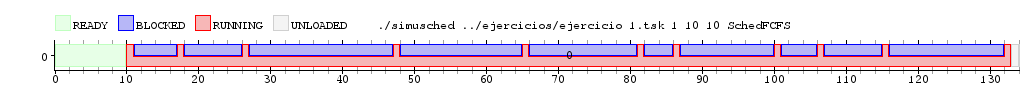
\includegraphics[width=15cm]{../ejercicios/ejercicio 1}
\end{figure}

\section{Ejercicio 2}

El lote de tareas para este ejercicio fue bastante simple, simplemente se compone de dos Tasks que corren desde un principio, el primero un TaskCPU de 100 ciclos, que representa al algoritmo complejo,y el segundo un TaskConsola (implementado en el ejercicio anterior) con 20 llamadas bloqueantes de entre 2 y 4 ciclos cada una, que representaría a la aplicación de musica. Y luego de 80 ciclos se carga otra TaskConsola con 25 llamadas bloqueantes de entre 2 y 4 ciclos cada una, que representa al navegador, para dar cuenta que esta ultima tarea se ejecuto luego de la aplicación de musica.

A continuación veremos como se comportó este lote al cargarse a través de un scheduler con política FCFS, en uno y dos núcleos respectivamente:

\begin{figure}[h!]
\caption{Lote de tareas ejecutándose en 1 núcleo \label{grf:ex2-1}}
\centering
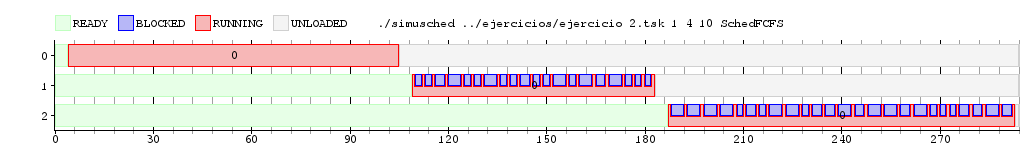
\includegraphics[width=15cm]{../ejercicios/ejercicio 2 - 1 nucleo}
\end{figure}

\begin{figure}[h!]
\caption{Lote de tareas ejecutándose en 2 núcleos \label{grf:ex2-2}}
\centering
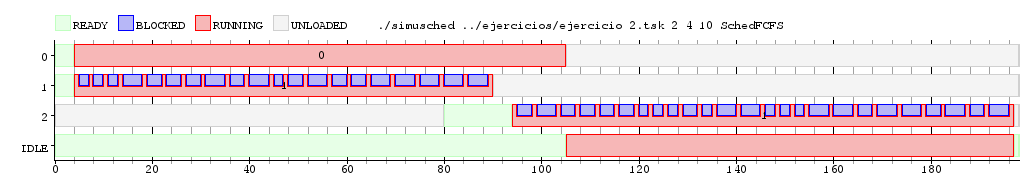
\includegraphics[width=15cm]{../ejercicios/ejercicio 2 - 2 nucleos}
\end{figure}

Como se puede observar, lo que sucede con esta política al aplicarse sobre una maquina de un núcleo, es que se convierte en un planificador secuencial, lo cual es lógico ya que trabaja como una cola, y al haber solo un núcleo, las aplicaciones se van a ir desencolando a medida que se libere ese único núcleo.
Algo muy parecido se puede ver en el caso de planificación con dos núcleos, solo que ahora se puede desencolar para cada núcleo a medida que se liberen, lo que permite una ejecución paralela de tareas.\\
Los tiempos de latencia para la ejecución en un núcleo fueron:
\begin{itemize}
\item Algoritmo Complejo: 4 ciclos
\item Reproductor: 109 ciclos
\item Navegador: 183 ciclos
\end{itemize}

Y para dos núcleos:
\begin{itemize}
\item Algoritmo Complejo: 4 ciclos
\item Reproductor: 4 ciclos
\item Navegador: 77 ciclos
\end{itemize}

\section{Ejercicio 3}



\section{Ejercicio 5}
\section{Ejercicio 6}

\section{Ejercicio 7}

Comenzamos con el lote

\begin{verbatim}
TaskCPU 200
@20:
TaskCPU 200
\end{verbatim}

\begin{figure}[h!]
\caption{Primer lote de tareas \label{grf:ex7-1}}
\centering
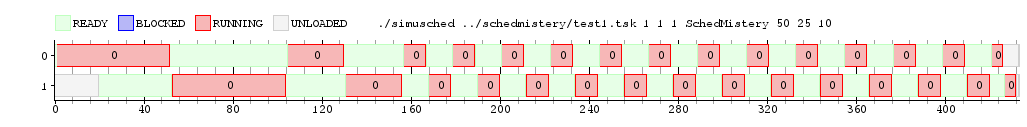
\includegraphics[width=15cm]{../ejercicios/ejercicio 7-1}
\end{figure}

Utilizando todos los argumentos del programa en 1, y pasando como único argumento del scheduler al 1 también. Luego probamos con pasar 5, 10, y después comenzamos a agregar argumentos. Esto nos permitió darnos cuenta que el quantum de tiempo para las tareas debía corresponderse con los argumentos. Luego, utilizamos el siguiente lote de tareas:

\begin{figure}[h!]
\caption{Resultado del segundo lote de tareas \label{grf:ex7-2}}
\centering
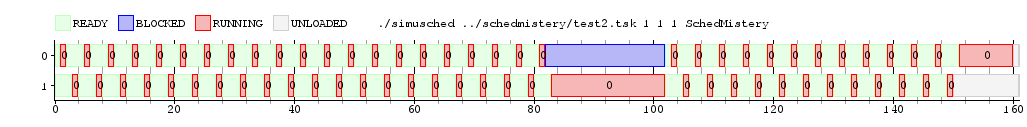
\includegraphics[width=15cm]{../ejercicios/ejercicio 7-2}
\end{figure}

\begin{verbatim}
TaskAlterno 20 20 20
TaskCPU 50
\end{verbatim}

Que nos mostró que el scheduler de la cátedra baja el quantum de los procesos al valor anterior cuando se bloquean, así como que el primer quantum debe ser uno. Finalmente, testeamos que este andando bien corriendo varios ejemplos, que se pueden encontrar en la carpeta \verb`schedmistery`.

\section{Ejercicio 8}

\end{document}